% rubber: module pdftex
% rubber: path HY

%%%%%%%%%%%%%%%%%%%%%%%%%%%%%%%%%%%%%%%%%%%%%%%%%%%%%%%%%%
%  Usage HOWTO                                           %
%  -----------                                           %
%  * Compilation:          rubber presentation           %
%  * Cleaning:             rubber --clean presentation   %
%  * Force recompilation:  rubber --force presentation   %
%%%%%%%%%%%%%%%%%%%%%%%%%%%%%%%%%%%%%%%%%%%%%%%%%%%%%%%%%%

\documentclass[t,12pt,pdftex]{beamer}
\usepackage{helvet}
\usepackage{times}
\usepackage{courier}

\usepackage[T1]{fontenc}
\usepackage[english]{babel}

\usepackage{amssymb}
\usepackage{amsmath}
\usepackage{amsfonts}
\usepackage{graphicx}
\usepackage{color}
\usepackage{url}
\usepackage{textpos}
\usepackage{xspace}
\usepackage{array}
\usepackage{longtable}

\graphicspath{{./fig/}}

% theme options: hy/ml/hum, rovio/sinetti, hiit
% default: hy,rovio

%\usetheme[hy]{HY}
%\usetheme[hy,sinetti]{HY}
%\usetheme[hum,rovio]{HY}
\usetheme[ml,rovio]{HY}
%\usetheme[ml,rovio,hiit]{HY}


\title{Automated tools for source code plagiarism detection}
%\author{Name Name \scriptsize \guilsinglleft{}name.name@helsinki.fi\guilsinglright{}}
\author{Kristian Wahlroos}
\institute{University of Helsinki\\Department of Computer Science}
\date{\today}

\begin{document}

%\selectlanguage{english}

\HyTitle

\begin{frame}
	\frametitle{Outline}
	\tableofcontents
\end{frame}


%\AtBeginSection[]
%{
%  \begin{frame}<beamer>
%    \frametitle{Outline}
%    \tableofcontents[currentsection]
%  \end{frame}
%}

\section{Introduction}

\subsection{Problem}

\begin{frame}
	\frametitle{Introduction}
	
	\begin{itemize}
		\item MOOC's have gained popularity in recent years
		\begin{itemize}
			\item Especially programming related MOOC's\footnote{\url{http://blog.edx.org/10-most-popular-courses-edx-courses-in-2016}}
			\item Independent assignments
			\item No live-presence required
		\end{itemize}
		\item Number of students often large
		\item Trust is thus usually one-sided
		\begin{itemize}
			\item Belief that students do tasks by themselves
			\item Not actively monitored
			\item Cheating is in form of plagiarism
			\item Many potential plagiarism scenarios
		\end{itemize} 
	\end{itemize}
\end{frame}

\subsection{Plagiarism}


\begin{frame}
	\vspace{1in}
	\begin{itemize}
			\item Source code plagiarism is a problem consisting many forms
		\begin{itemize}
			\item Straight plagiarism
			\item Too intense group work 
			\item Code sharing
			\item Obfuscation
		\end{itemize}
		\item Lots of students $\rightarrow$ impossible to detect manually in reasonable time
		\begin{itemize}
			\item Lot of data available
			\item Need for automated tools
		\end{itemize}
	\end{itemize}
\end{frame}

\subsection{Motivation}

\begin{frame}
	\frametitle{In this study}
	\begin{itemize}
		\item Finding a suitable machine learning tool set for detecting source code plagiarism
		\item Motivated by
		\begin{itemize}
			\item Could be used in University of Helsinki's course \textit{Introduction to programming}
			\item Interesting topic
			\item Machine learning methods benefit from a lot of data
		\end{itemize}
		\item Results reflected to the usage in a academic course
	\end{itemize}
\end{frame}




\section{Methodology}
\subsection{Literature review}


\begin{frame}
	\frametitle{Methodology}
	\begin{itemize}
		\item Performing literature review with \textit{Google Scholar}
		\item Collected 8 papers 
		\item Two-step search process
		\begin{itemize}
			\item Limit by overall keywords occurrences
			\item Limit by title/abstract/keywords
		\end{itemize}
		\item Keywords
		\begin{itemize}
			\item Direct matches: \textbf{machine learning, plagiarism, code, programming}
			\item Non-direct: \textbf{authorship, identification} 
		\end{itemize}
	\end{itemize}
\end{frame}

\begin{frame}
	\vspace{1in}
	\begin{itemize}
		\item Limited years starting from 2006
		\begin{itemize}
			\item Believed to contain more recent programming languages
			\item MOOC's are relatively new concept
			\item Machine learning methods have changed
		\end{itemize}
		\item Doing comparison between papers
		\begin{itemize}
			\item Model accuracy
			\item Data
			\item Machine learning methodology
			\item Feature extraction
		\end{itemize}
	\end{itemize}
\end{frame}

\section{Results}
\subsection{Overview}
\begin{frame}
	\frametitle{Results}
	\begin{itemize}
		\item 8 papers from 2007 to 2015
		\begin{itemize}
			\item[1)] \textit{A machine learning based tool
for source code plagiarism detection}, 2011
			\item[2)] \textit{De-anonymizing
programmers via code stylometry}, 2015
			\item[3)] \textit{Detecting outsourced student
programming assignments}, 2008
			\item[4)] \textit{Pde4java: Plagiarism detection
engine for java source code: a clustering approach}, 2008
		\end{itemize}
	\end{itemize}
\end{frame}

\begin{frame}
	\vspace{0.5in}
	\begin{itemize}
	\item[5)] \textit{A probabilistic approach to source code authorship identification}, 2007
			\item[6)] \textit{Using code metric histograms and genetic algorithms to perform author identification for software forensics}, 2007
			\item[7)] \textit{Who wrote
this code? Identifying the authors of program binaries}, 2011
			\item[8)] \textit{An application for plagiarized source code detection based on a parse
tree kernel}, 2013
	\end{itemize}
\end{frame}

\begin{frame}
	\vspace{0.5in}
	\begin{itemize}
		\item Studies divide into two categories
		\begin{itemize}
			\item Attribute counting (4 papers)
			\item Structure based (4 papers)
		\end{itemize}
		\item Attribute counting is easy and fast $\rightarrow$ directly from the source code
		\item Structure based require parsing
		\item Model accuracies are reported in two ways
		\begin{itemize}
			\item Traditional classification accuracy
			\item How close the model was to human labeling
		\end{itemize}
	\end{itemize}
\end{frame}

\begin{frame}
	\vspace{0.5in}
	\begin{itemize}
		\item Accuracies ranged from 69\% to over 90\%
		\begin{itemize}
			\item Highest used mixture of stylistic and structural approach
			\item E.g. 93\% same results compared to human validator
		\end{itemize}
		\item Plagiarism detection is close to authorship identification
			\begin{itemize}
			\item Classifying anonymous source code
			\item Clustering similar documents together
			\item Finding stylistic nuances
			\item Trying to capture the logical structure
		\end{itemize}
	\end{itemize}
\end{frame}

\subsection{Data}

\begin{frame}
	\begin{itemize}
		\frametitle{Data sets in studies}
		\item No clear difference between stylistic studies and structural studies
		\begin{itemize}
			\item Partially reported data sets
			\item Just few authors in stylistic studies
		\end{itemize}
	\end{itemize}

\begin{table}[ht]
\centering
\scalebox{0.8}{
\begin{tabular}{c|cccccccc}
\textbf{Attr./Paper} & 1   & 5   & 3  & 6    & 8   & 2    & 4   & 7   \\ \hline
\textbf{Size}        & 741 & 200 & 83 & 4068 & 555 & N/A  & 326 & 203 \\
\textbf{Authors}     & 10  & 8   & 12 & 20   & N/A & 1600 & N/A & 32\\ 
\textbf{Structural} &No&No&No&No&Yes&Yes&Yes&Yes
\end{tabular}
}
\caption{Reported data sets used in papers}
\label{table:data}
\end{table}
\end{frame}

\begin{frame}
	\vspace{0.5in}
	\begin{itemize}
		\item Data sets are often collected from course assignments
		\item Open source projects are utilized to gather the data set
		\item Competitions
		\begin{itemize}
			\item \textit{Google Code Jam}
			\item Explains the large number of possible authors
		\end{itemize}
	\end{itemize}
\end{frame}

\subsection{Methodologies}

\begin{frame}
	\frametitle{Machine learning methods}
	
\begin{table}[ht]
\centering
\scalebox{0.7}{
\begin{tabular}{c|cccccccc}
\textbf{Attr./Paper} & 1   & 5   & 3  & 6    & 8   & 2    & 4   & 7   \\ \hline
\textbf{Method}        & $E_3$ & NB/VFI & DT & GA & PTK & RF  & DM & K-M/SVM \\
\textbf{Structural} &No&No&No&No&Yes&Yes&Yes&Yes
\end{tabular}
}
\caption{Methods used in studies}
\label{table:meth}
\end{table}	

\begin{footnotesize}
\begin{longtable}{ll}

{$\mathbf{E_i}$} & Ensemble of i models \\
\textbf{NB} & Naive Bayes\\
\textbf{VFI} & Voting Feature Interval\\
\textbf{DT} & Decision Tree\\
\textbf{GA} & Genetic Algorithm\\
\textbf{PTK} & Parse Tree Kernel\\
\textbf{RF} & Random Forest\\
\textbf{DM} & Data Mining (DBSCAN)\\
\textbf{K-M} & K-means Clustering\\
\textbf{SVM} & Support Vector Machine

\end{longtable}
\end{footnotesize}

\end{frame}

\begin{frame}
	\vspace{0.5in}
	\begin{itemize}
	\item Many various algorithms used
	\begin{itemize}
		\item Probabilistic 
		\item Trees
		\item Genetic algorithm
		\item Clustering
	\end{itemize}
	\item Structural studies tend to favor tree-structures and clustering
	\begin{itemize}
		\item Easy due to nature of code structure
		\item Overcomes the obfuscation
		\item Pre-parsing often required
	\end{itemize}
	\item More variance in stylistic studies 
	\begin{itemize}
		\item Probabilistic models
		\item Genetic algorithm
		\item Decision tree
	\end{itemize}
	\end{itemize}
\end{frame}

\subsection{Feature extraction}

\begin{frame}
	\frametitle{Features}
	\begin{itemize}
		\item \textit{How source code is transformed to feature vector?}
		\item {\textit{How similarity is being measured?}}
		\item Inspected from two viewpoints
		\begin{itemize}
			\item Attribute counting (stylistic)
			\item Structural
		\end{itemize}
		\item Most stylistic studies extract the features directly from the source code
		\item Structural studies tend to parse the document and use abstract syntax tree as a base for features
	\end{itemize}
\end{frame}

\begin{frame}
	\frametitle{Features - stylistic}
	\begin{itemize}
		\item[1)] \textit{A machine learning based tool
for source code plagiarism detection}, 2011
		\begin{itemize}
			\item Code as set of tokens
			\item Parsing with ANTLR-parser
			\item 9 different metrics
			\begin{itemize}
				\item Number of characters per line
				\item Number of words in document
				\item Number of access modifiers	
			\end{itemize}
		\end{itemize}
	\end{itemize}
\end{frame}

\begin{frame}
	\vspace{0.5in}
	\begin{itemize}
		\item[5)] \textit{A probabilistic approach to source code authorship identification}, 2007
		\begin{itemize}
			\item Three step pipeline
			\begin{itemize}
				\item[I)] Extract metrics
				\item[II)] Filter metrics
				\item[III)] Form writer profiles
			\end{itemize}
			\item Style and pattern based metrics
			\begin{itemize}
				\item Style consists line sizes, leading spaces and commas as distributions
				\item Pattern based is distribution of possible N-grams
			\end{itemize}
			\item 4 was considered as the best length in N-gram
		\end{itemize}
	\end{itemize}
\end{frame}

\begin{frame}
	\vspace{0.5in}
	\begin{itemize}
		\item[3)] \textit{Detecting outsourced student
programming assignments}, 2008
		\begin{itemize}
			\item Programmer profiles (writer profiles)
			\item Utilizing \textit{Weka} to parse documents
			\item Six metrics
			\begin{itemize}
				\item zipped size
				\item lines of code
				\item number of variables
				\item number of for-loops
				\item number of comments
				\item variable lengths
			\end{itemize}
		\end{itemize}
	\end{itemize}
\end{frame}

\begin{frame}
	\vspace{0.5in}
	\begin{itemize}
		\item[6)] \textit{Using code metric histograms and genetic algorithms to perform author identification for software forensics}, 2007
		\begin{itemize}
			\item 18 base metrics 
			\item Gathered metric values are transformed into distributions
			\item Text-based and syntactic metrics
			\item Genetic algorithm to find the best combination
			\begin{itemize}
				\item usage of curly braces
				\item comment amount and style
				\item indentation
				\item inline spaces
				\item length of lines
				\item switch-cases
				\item control flows (if-else)
				\item frequencies of first characters in variables
			\end{itemize}
		\end{itemize}
	\end{itemize}
\end{frame}


\begin{frame}
	\frametitle{Features - structural}
	\begin{itemize}
		\item[8)] \textit{An application for plagiarized source code detection based on a parse
tree kernel}, 2013
	\begin{itemize}
		\item Parse tree kernel
		\begin{itemize}
			\item Produces similarities between source codes
			\item Tree kernels are used often in linguistics
		\end{itemize}
		\item Similarity matrix to group source codes 
		\item Utilizing heavily the tree structure
	\end{itemize}
	\end{itemize}
\end{frame}

\begin{frame}
	\begin{figure}[ht]
			\centering
			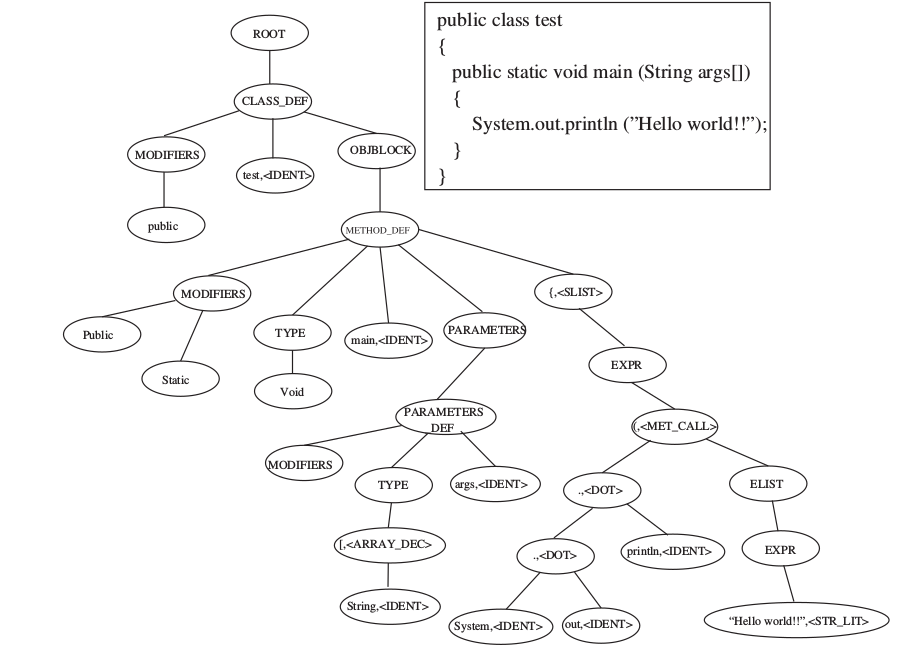
\includegraphics[scale=0.3]{parse_tree}	
			\caption{Example of parse tree in study 8}
	\end{figure}
\end{frame}

\begin{frame}
	\vspace{0.5in}
	\begin{itemize}
		\item[2)] \textit{De-anonymizing
programmers via code stylometry}, 2015
		\begin{itemize}
			\item Building \textit{Code Stylometry Feature Set}
			\item Utilizing abstract syntax tree (AST)
			\item 3 classes of features used
			\begin{itemize}
				\item Lexical (number of functions/keywords)
				\item Layout (indentation, whitespace)
				\item Syntactic (maximum depth of AST, AST bigrams)
			\end{itemize}
		\end{itemize}
	\end{itemize}
\end{frame}

\begin{frame}
	\vspace{0.5in}
	\begin{itemize}
		\item[4)] \textit{Pde4java: Plagiarism detection
engine for java source code: a clustering approach}, 2008
		\begin{itemize}
			\item Source code into n-grams via tokenization
			\item 4-grams 
			\item Similarity measure by \textit{Jaccard coefficient}
			\begin{itemize}
				\item In simplified form: ratio of specific n-gram between two documents
			\end{itemize}
			\item Similarity is used to group documents into clusters
		\end{itemize}
	\end{itemize}
\end{frame}

\begin{frame}
	\vspace{0.5in}
	\begin{itemize}
		\item[7)] \textit{Who wrote
this code? Identifying the authors of program binaries}, 2011
		\begin{itemize}
			\item Graphs and N-grams as features
			\item Binary code first into machine language
			\item Flow graphs
			\begin{itemize}
				\item Idioms: short instruction sequences
				\item Graphlets: local structure of the program
				\item Supergraphlets: combine graphlets and simplify
				\item Call graphlets: interaction between external libraries
			\end{itemize}
			\item N-grams size of 4-bytes is used
		\end{itemize}
	\end{itemize}
\end{frame}


\section{Discussion}

\begin{frame}
	\frametitle{Recap}
	\begin{itemize}
		\item Two distinctions between studies: stylistic and structural
		\begin{itemize}
			\item Stylistic is can be gained directly from the source code
			\item Structure deals with tree-like data
		\end{itemize}
		\item Data is quite easily obtainable
		\begin{itemize}
			\item Open-source projects
			\item Competitions
			\item Courses inside universities
		\end{itemize}
		\item It all comes down to author identification
		\begin{itemize}
			\item \textit{Who wrote this code?}
		\end{itemize}
	\end{itemize}
\end{frame}

\begin{frame}
	\frametitle{Criticism}
	\begin{itemize}
		\item Some papers are not reporting explicitly the data and author counts
		\item No justification/comparing between different machine learning models
		\item Detection model is rarely put into real life test
		\begin{itemize}
			\item No proof of the actual (real-life) performance
			\item Plagiarism accusation is difficult topic
			\item What to do if task is very limited
		\end{itemize}
	\end{itemize}
\end{frame}

\begin{frame}
	\frametitle{Reflection - \textit{Introduction to Programming}}
	\begin{itemize}
		\item Six weeks of assignments 1 machine test		
		\item Based on study 2
		\begin{itemize}
			\item 3 classes of features: lexical, stylistic and syntactic
			\item Classifying 250 programmers should give good quite accurate results	
		\end{itemize}
		\item Training the model (programmer profiles) for six weeks
		\item Testing against unseen data $\rightarrow$ machine test	 		\item If model would alarm, requires manual step
	\end{itemize}
\end{frame}

\begin{frame}
	\vspace{1.5in}
	Thank you
\end{frame}

\end{document}
